\subsection{Robot e-puck} \label{sec:robot_epuck}

Le robot e-puck2 est une évolution du robot éducatif e-puck, développé conjointement par GCtronic et l'EPFL.
Il est conçu pour l'enseignement et la recherche en robotique, offrant une plateforme compacte et polyvalente \autocite{gctronic_e-puck2_nodate}.

\begin{figure}[H]
    \centering
    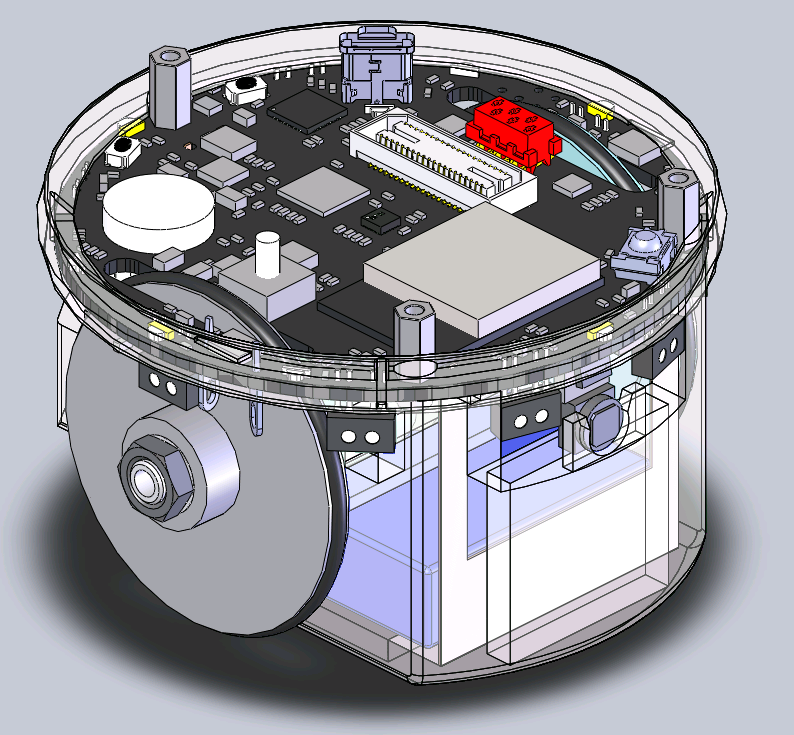
\includegraphics[width=0.5\linewidth]{figures//e-puck2_image3D.png}
    \caption{Représentation 3D d'un e-puck2 par GCTronic \autocite{noauthor_gctronic_nodate}}
    \label{fig:epuck2_3Dschema}
\end{figure}

\subsubsection{Caractéristiques principales}
L'e-puck2 est équipé de divers capteurs et actionneurs.
Ces composants lui permettent de réaliser une variété d'expériences en robotique, de la simple navigation à des interactions complexes avec l'environnement \autocites{gctronic_e-puck2_nodate}{noauthor_gctronic_nodate}.

\paragraph{Capteurs}
Le robot dispose des capteurs suivants pour interagir avec son environnement : 
\begin{itemize} 
    \item 8 capteurs de proximité et de lumière ambiante pour détecter les obstacles et mesurer les distances ;
    \item 1 capteur de distance Time-of-Flight pour des mesures de distance plus précises allant jusqu'à 2 mètres ;
    \item 1 \acrfull{imu} 3D, un ensemble de capteurs inertiels à 9 axes pour mesurer l'accélération, la rotation et l'orientation \autocite{noauthor_inertial_2025} ; 
    \item 4 microphones omnidirectionnels pour la capture du son ;
    \item 1 caméra couleur VGA ;
    \item 1 récepteur infrarouge pour le contrôle à distance.
\end{itemize}

\paragraph{Moteurs}
Il est équipé de deux moteurs à courant continu avec encodeurs pour un contrôle précis du mouvement.  

\paragraph{Sorties}
Pour la communication visuelle et auditive, l'e-puck2 est doté de : 
\begin{itemize}
    \item 4 \acrshort{led}s rouges ;
    \item 4 \acrshort{led}s RGB ;
    \item 1 lumière verte sur le corps ;
    \item 1 \acrshort{led} rouge puissante à l'avant ;
    \item 1 haut-parleur capable de lire des fichiers \acrshort{wave}.
\end{itemize}

\paragraph{Alimentation}
Il est alimenté par une batterie Li-Ion de 1.8 Ah, offrant une autonomie d'environ 3 heures.

\paragraph{Communication}
Le robot prend en charge plusieurs modes de communication : 
\begin{itemize} 
    \item USB Full-speed pour la programmation, le transfert de données et la recharge de la batterie ;
    \item Bluetooth 2.0 et \acrfull{ble} pour la connectivité sans fil avec des ordinateurs ou appareils mobiles ;
    \item Wi-Fi pour les communications réseau avancées.
\end{itemize}

\subsubsection{Extensions pour le robot}

\begin{figure}[H]
    \centering
    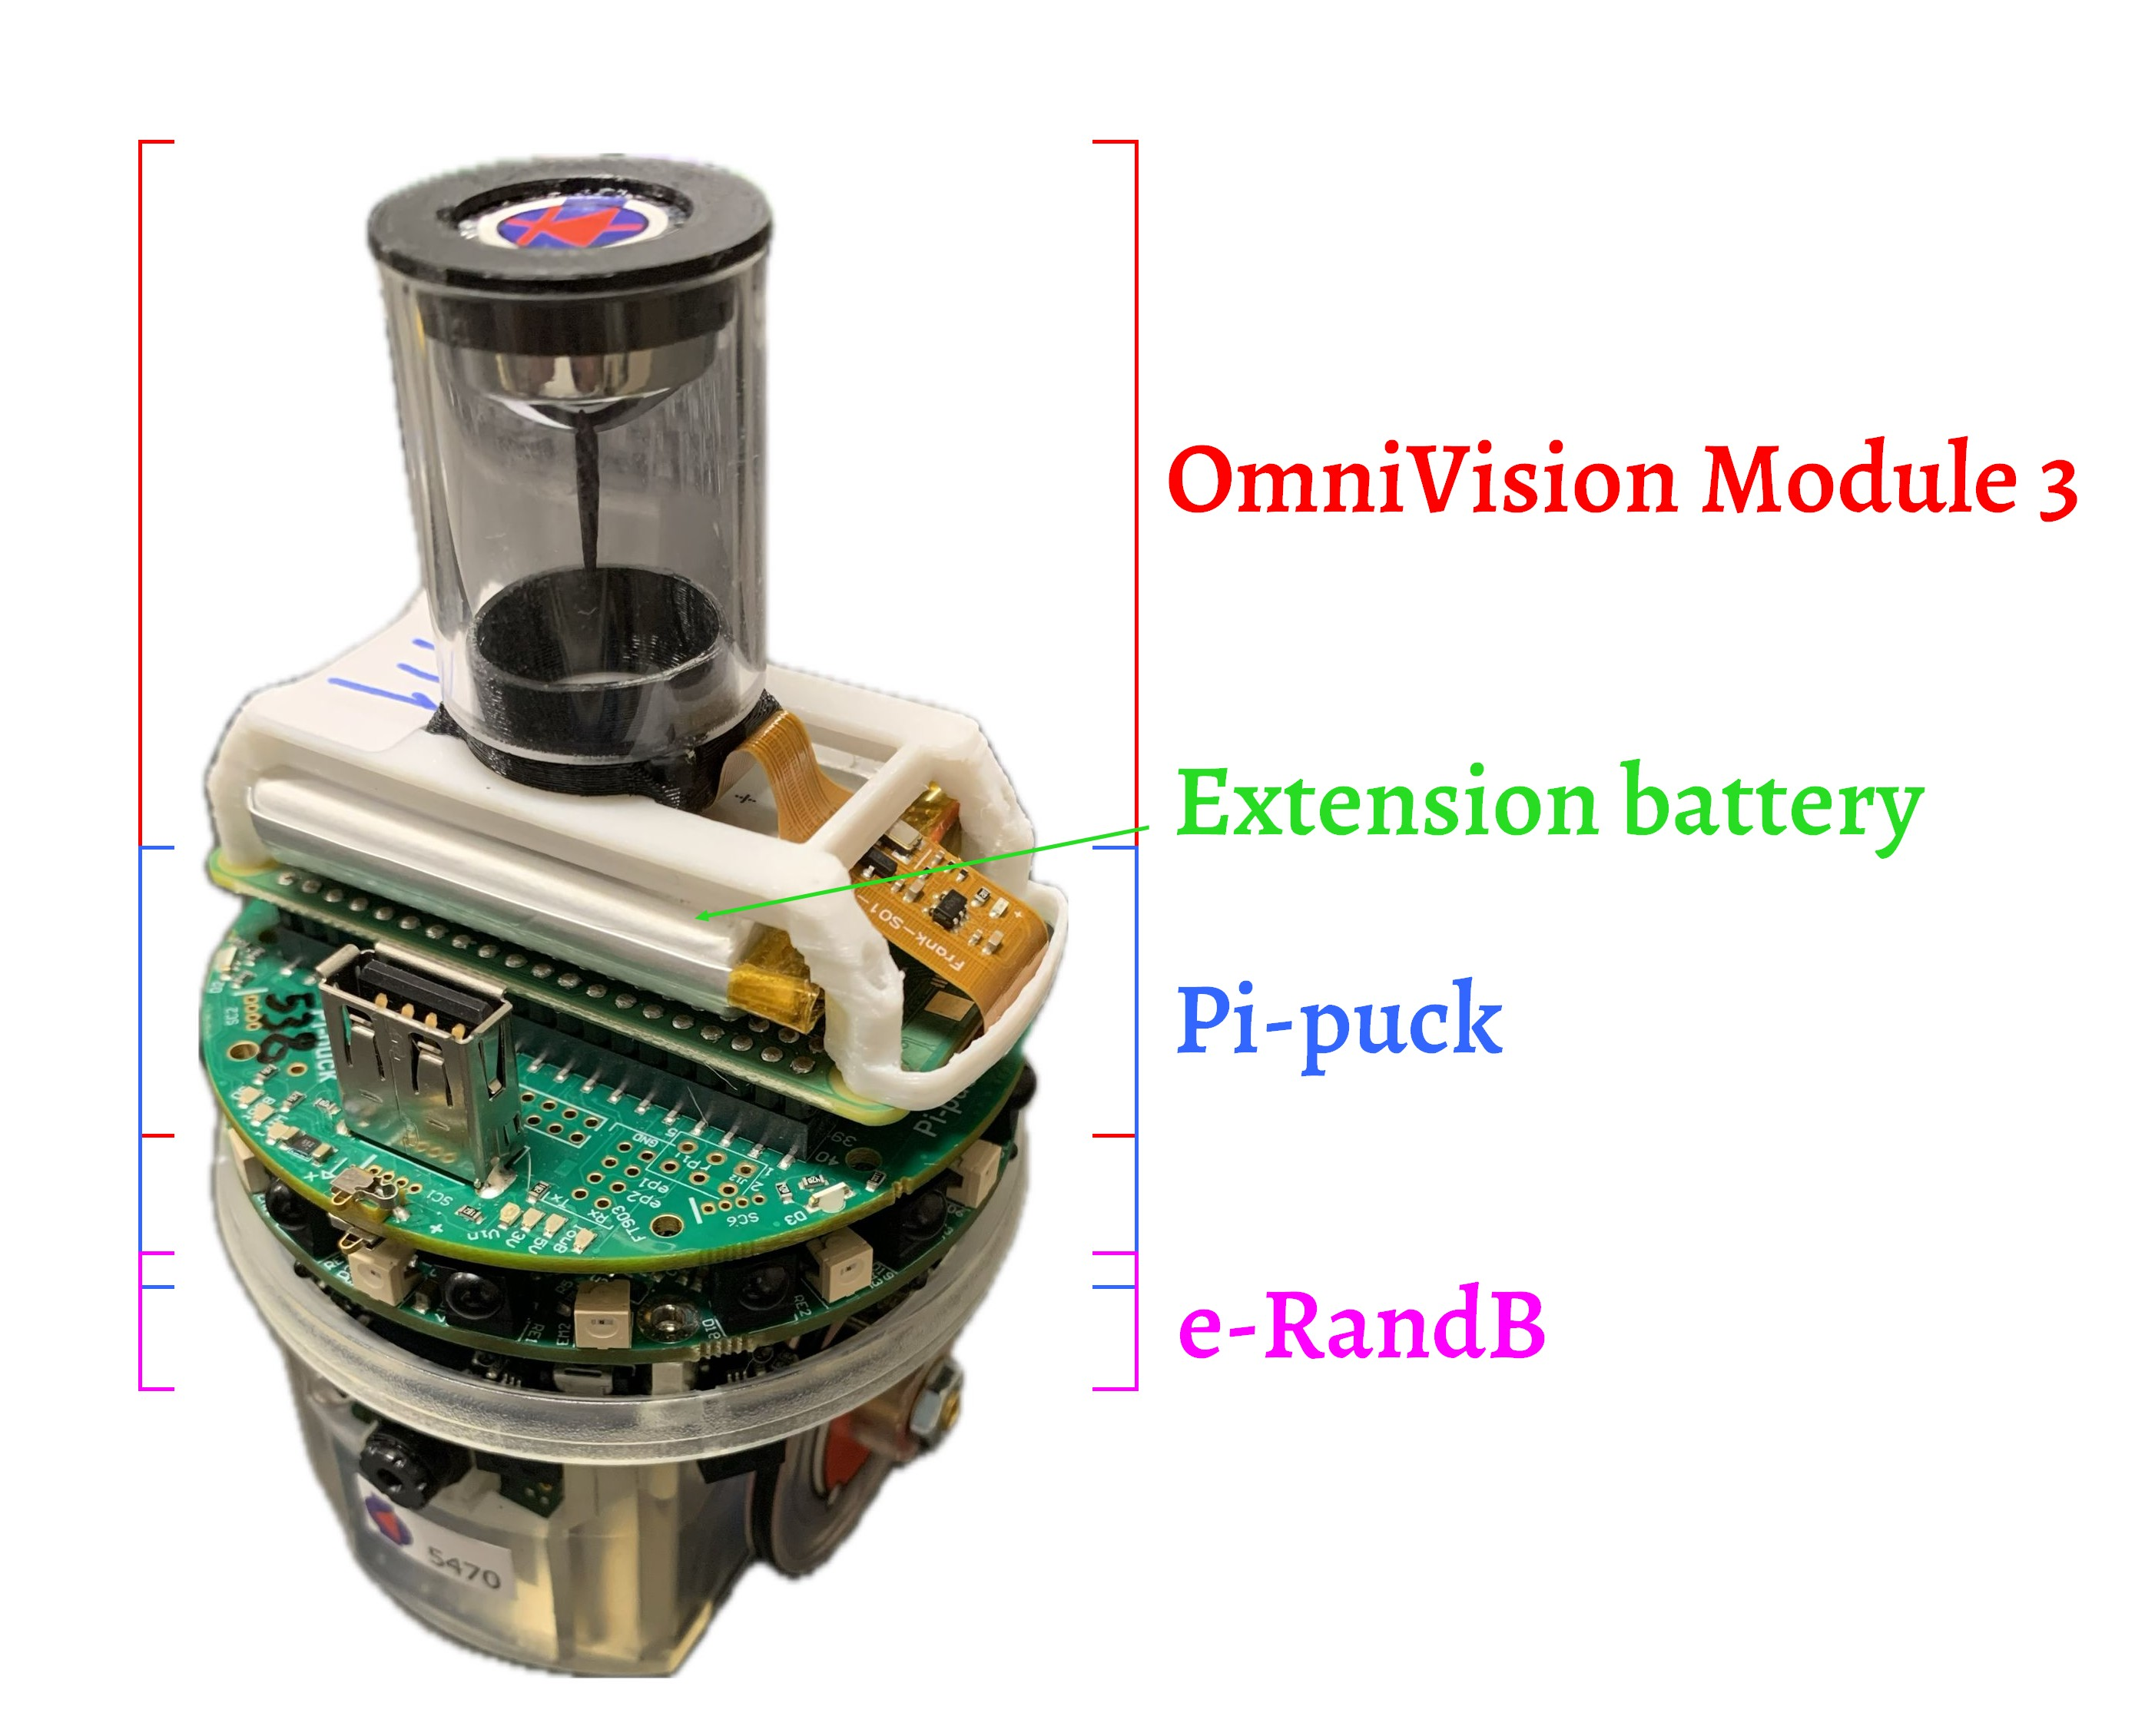
\includegraphics[width=0.75\linewidth]{figures//epuck2_rangeandbearing_epuck_omnivisioncam3_highlighted.jpg}
    \caption{Photo d'un e-puck2 avec les extensions attachées}
    \label{fig:epuck2_unamur}
\end{figure}

\paragraph{Pi-puck}
Le Pi-puck est une extension matérielle qui intègre un Raspberry Pi Zero W ou Zero 2 W au robot e-puck2, élargissant ses capacités de calcul et de connectivité.
Cette combinaison permet d'exécuter des applications plus complexes, telles que la vision par ordinateur, le traitement avancé des données et l'apprentissage automatique \autocite{gctronic_pi-puck_nodate}.

\paragraph{\acrshort{erandb}}
Le \acrfull{erandb} est une extension pour l'e-puck2 qui améliore les capacités de communication et de localisation relative entre robots.
Cette carte permet aux robots de communiquer localement tout en obtenant simultanément la distance et la direction de l'émetteur, sans nécessiter de contrôle centralisé ou de référence externe \autocite{gctronic_range_nodate}.
L'\acrshort{erandb} est particulièrement utile dans les recherches en robotique en essaim, où la communication et la localisation relative entre robots sont essentielles \autocites{almansoori_evolution_2022}{vitanza_robot_2019}.

\paragraph{OmniVision Module 3}
L'OmniVision Module 3 est un module pour l'e-puck2 intégrant un câble flexible et une caméra grand angle miniature (OmniVision5647).
Combiné à un miroir parabolique, cette caméra est attachée à un cône transparent sur une impression 3D conçue sur mesure pour le Pi-puck \autocite{noauthor_omnivision_nodate}.
Il permet de fournir des capacités de vision omnidirectionnelle à l'e-puck.

\paragraph{Batterie externe supplémentaire}
Une batterie d'extension de 1.5 Ah a été ajoutée au système afin d'augmenter la capacité totale du robot.

\subsubsection{Présentation générale du projet}
Grâce à ses capteurs variés et ses différentes extensions matérielles, l'e-puck2 constitue une plateforme robotique polyvalente adaptée à l'enseignement et à la recherche.
Ces améliorations font de l'e-puck2 un robot modulaire, capable d'évoluer en fonction des besoins pédagogiques et des applications robotiques avancées.

Cependant, bien que ses capacités techniques soient riches, l'utilisation de l'e-puck2 reste complexe et peu accessible au public visé.
C'est pourquoi ce mémoire vise à créer une interface intuitive adaptable à différents niveaux d'apprentissage :
\begin{enumerate}
    \item \textbf{Enfants (6-12 ans)} : une interface ludique et intuitive ;
    \item \textbf{Adolescents (13-18 ans)} : un environnement plus structuré, intégrant des concepts avancés comme la logique algorithmique et la programmation robotique.
\end{enumerate}

L’objectif d'une telle interface est de permettre la réalisation de trois grandes catégories d’actions, définies comme suit par le Dr. Tuci.  

\begin{itemize}
    \item \textbf{Navigation} : exécution de parcours pré-définis, comme la traversée d’un labyrinthe.
    
    \item \textbf{Exploration} : recherche et identification d’éléments spécifiques dans l’environnement, tels que des dalles de couleur.
    
    \item \textbf{Observation de comportements collectifs}\footnote{Comme indiqué en \autoref{sec:limites}, cette catégorie dépasse le cadre du présent projet, en raison des contraintes liées à la coordination multi-robots. Elle est néanmoins présentée ici afin d’offrir une vision d’ensemble et de justifier certains choix techniques facilitant son intégration future.} : mise en relation de plusieurs robots afin d’observer des interactions coordonnées, par exemple dans un scénario de type "jeu du chat et de la souris".
\end{itemize}

Les trois paragraphes suivants détaillent chacune de ces catégories d'actions.

\paragraph{Navigation}
Ce mode consiste à guider le robot selon un parcours précis, comme traverser un labyrinthe ou se déplacer dans une arène délimitée.
Les déplacements peuvent être générés de manière aléatoire ou suivre un itinéraire prédéfini.
Ce mode nécessite la maîtrise des systèmes de locomotion du robot : moteurs, roues et capteurs de proximité pour la détection d’obstacles.

\paragraph{Exploration}
Dans ce mode, le robot doit rechercher des éléments visuellement identifiables, comme des zones blanches sur un sol noir.
Les trajectoires peuvent également être aléatoires ou définies à l’avance.
Ce mode implique des exigences matérielles plus importantes : capteurs infrarouges au sol, caméra embarquée, et traitement d’image pour l’identification des couleurs.

\paragraph{Observation de comportements collectifs}
Ce mode vise à faire interagir plusieurs robots simultanément, par exemple à travers des scénarios collaboratifs ou compétitifs.
Un robot peut être programmé pour suivre ou fuir un autre, selon des règles simples.
Cela implique la gestion de la communication inter-robots et la coordination de leurs actions dans un espace partagé.
